\documentclass[11pt]{article}
\usepackage[margin=1in]{geometry}
\usepackage{amsmath,amssymb,amsthm}
\usepackage{enumitem}
\usepackage{xcolor}
\usepackage{titlesec}
\usepackage{tikz}

\definecolor{defbg}{RGB}{176,109,120}
\definecolor{noteblue}{RGB}{90,140,200}
\definecolor{notepink}{RGB}{210,110,140}
\definecolor{noteyellow}{RGB}{170,140,40}

\titleformat{\section}{\normalfont\Large\bfseries}{\thesection}{1em}{}
\titleformat{\subsection}{\normalfont\large\bfseries}{\thesubsection}{1em}{}

\newcommand{\deftitle}[1]{%
  \vspace{0.6em}
  \noindent\colorbox{defbg!70}{\parbox{\dimexpr\textwidth-2\fboxsep}{\textbf{\textcolor{white}{#1}}}}
  \vspace{0.4em}
}

\newenvironment{note}{\begin{quote}\color{noteblue}\itshape}{\end{quote}}
\newenvironment{remark}{\begin{quote}\color{notepink}}{\end{quote}}
\newenvironment{proofnote}{\begin{quote}\color{noteyellow}}{\end{quote}}

\title{\textbf{Probability Measure}}
\author{Lecture 2 Notes}
\date{}

\begin{document}
\maketitle

\deftitle{Definition 2.1 --- Sample Space}

A sample space $\Omega$ is any non-empty set.

\vspace{0.5em}
\noindent \textbf{Example 2.1:} The sample space contains ``all the states of the following'':
\begin{itemize}
  \item Coin flipping: $\Omega = \{H, T\}$
  \item Weather: $\{\text{hot, cold, mild}\} \times \{\text{wet, dry}\}$
\end{itemize}

\deftitle{Definition 2.2 --- Probability Measure (STA 347 version)}

For a sample space $\Omega$, we say $P$ is a \textbf{probability measure} if the following hold:

\begin{enumerate}[label=(\roman*)]
  \item $\forall E \subseteq \Omega,\ 0 \le P(E) \le 1$, that is $P: \mathcal{P}(\Omega) \to [0,1]$ \hfill {\small\textcolor{noteblue}{$\leftarrow$ the power set}}
  \item $P(\Omega) = 1$
  \item $\forall E_1, E_2, \ldots \subseteq \Omega$ such that $E_i \cap E_j = \emptyset\ (\forall i \ne j)$ \hfill {\small\textcolor{noteyellow}{(mutually exclusive)}}
  \[
  P\Big(\bigcup_{i=1}^{\infty} E_i\Big) = \sum_{i=1}^{\infty} P(E_i)
  \]
\end{enumerate}

\begin{remark}
\textbf{Remark:} It may be impossible for such a $P$ to exist. To define exactly which subsets we want $P$ to satisfy this axiom, that will require more advanced mathematical theories. For this course, we just assume such a $P$ is defined for all subsets of $\Omega$.
\end{remark}

\noindent \textbf{Example 2.2:} Probability of coin flipping.
\[
\Omega = \{H, T\}, \qquad \mathcal{P}(\Omega) = \big\{\, \emptyset,\ \{H\},\ \{T\},\ \{H,T\} \,\big\}
\]
\[
P: \quad \emptyset \longmapsto 0, \qquad \{H\} \longmapsto \tfrac{1}{2}, \qquad \{T\} \longmapsto \tfrac{1}{2}, \qquad \{H,T\} \longmapsto 1.
\]

\noindent \textbf{Example 2.3:} The uniform / Lebesgue measure.

Let $\Omega = [L, U]$ for some $L < U \in \mathbb{R}$.
\[
P\big([a,b]\big) = \frac{b-a}{U-L} \qquad \text{when } L \le a \le b \le U.
\]

\deftitle{Proposition 2.3}

The following properties are satisfied by any probability measure $P$:

\begin{enumerate}
  \item $\forall E \subseteq \Omega,\quad P(E^c) = 1 - P(E)$
  \item $P(\emptyset) = 0$
  \item $\forall E, F \subseteq \Omega$ such that $E \subseteq F,\quad P(E) \le P(F)$ \hfill {\small\textcolor{notepink}{``big event, big probability''}}
  \item $\forall E, F \subseteq \Omega,\quad P(E \cup F) = P(E) + P(F) - P(E \cap F)$
  \item $\forall E, F \subseteq \Omega,\quad P(E \cap F) = P(E) + P(F) - P(E \cup F)$
  \item $\forall E, F \subseteq \Omega,\quad P(F \setminus E) = P(F) - P(E \cap F)$
\end{enumerate}

\begin{proofnote}
\textit{Proof} via Def 1.2 (probability axioms).
\end{proofnote}

\deftitle{Lemma 2.4 --- Subadditivity}

For a sequence $E_1, \ldots, E_n \subseteq \Omega$,
\[
P\Big(\bigcup_{i=1}^{n} E_i\Big) \le \sum_{i=1}^{n} P(E_i).
\]

\begin{proofnote}
\textbf{Proof.} We define $F_i = E_i \setminus \displaystyle\bigcup_{j=1}^{i-1} E_j$.

\begin{center}
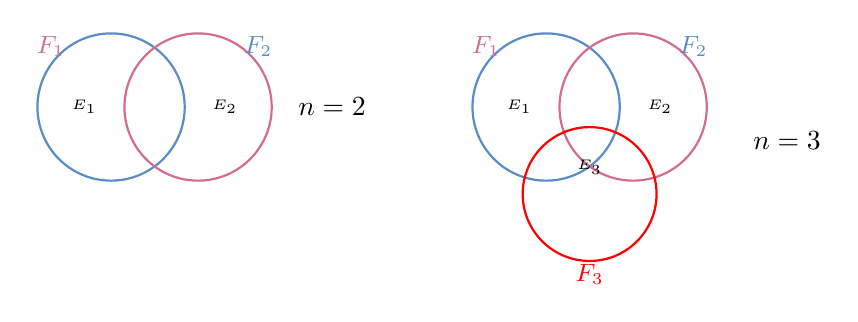
\begin{tikzpicture}[scale=0.85]
  % First diagram: F1, F2
  \begin{scope}
    \draw[thick, noteblue] (0,0) circle (1.1);
    \draw[thick, notepink] (1.3,0) circle (1.1);
    \node at (-0.9,0.9) {\small\textcolor{notepink}{$F_1$}};
    \node at (2.2,0.9) {\small\textcolor{noteblue}{$F_2$}};
    \node at (-0.4,0) {\tiny $E_1$};
    \node at (1.7,0) {\tiny $E_2$};
    \node at (3.3,0) {$n=2$};
  \end{scope}
  % Second diagram: F1, F2, F3
  \begin{scope}[xshift=6.5cm]
    \draw[thick, noteblue] (0,0) circle (1.1);
    \draw[thick, notepink] (1.3,0) circle (1.1);
    \draw[thick, red] (0.65,-1.3) circle (1.0);
    \node at (-0.9,0.9) {\small\textcolor{notepink}{$F_1$}};
    \node at (2.2,0.9) {\small\textcolor{noteblue}{$F_2$}};
    \node at (0.65,-2.5) {\small\textcolor{red}{$F_3$}};
    \node at (-0.4,0) {\tiny $E_1$};
    \node at (1.7,0) {\tiny $E_2$};
    \node at (0.65,-0.9) {\tiny $E_3$};
    \node at (3.6,-0.5) {$n=3$};
  \end{scope}
\end{tikzpicture}
\end{center}

Then
\[
\bigcup_{i=1}^{n} E_i = \bigcup_{i=1}^{n} F_i, \qquad \text{and} \qquad F_i \cap F_j = \emptyset \text{ if } i \ne j \quad \text{(mutually exclusive)}
\]
from the probability axioms. Since $\displaystyle\bigcup_{i=1}^{n} E_i = \bigcup_{i=1}^{n} F_i$ and $F_i \cap F_j = \emptyset$ for $i \ne j$,
\[
P\Big(\bigcup_{i=1}^{n} E_i\Big) = P\Big(\bigcup_{i=1}^{n} F_i\Big) = \sum_{i=1}^{n} P(F_i).
\]
We also know $F_i \subseteq E_i$ (as $F_i = E_i \setminus \bigcup_{j=1}^{i-1} E_j$), so $P(F_i) \le P(E_i)$. Hence
\[
P\Big(\bigcup_{i=1}^{n} E_i\Big) = \sum_{i=1}^{n} P(F_i) \le \sum_{i=1}^{n} P(E_i). \qquad \blacksquare
\]
\end{proofnote}

\deftitle{Lemma 2.5}

Let $P$ be the Lebesgue measure on $[0,1]$. Then $P(E) = 0$ for any countable set $E$.

\end{document}
